\documentclass[a4paper]{article}
\usepackage{cmap}
\usepackage{mathtext}
\usepackage{amssymb}
\usepackage{amsmath}
\usepackage{wrapfig}
\usepackage[russian]{babel}
\usepackage{indentfirst}
\usepackage[pdftex]{graphicx}
\usepackage{multirow}
\usepackage{mathrsfs}
\usepackage{biblatex}
\usepackage{siunitx}
\usepackage[left=2cm,right=2cm,top=2cm,bottom=2cm]{geometry}
\usepackage{fancyhdr}
\bibliography{bib}
\pagestyle{fancy}
\newcommand{\const}{\mathrm{const}}
\newcommand{\rref}[1]{(\ref{#1})}
\newcommand{\isotope}[2]{$ ^{#2}\mathrm{#1} $}
\newenvironment{comment}{}{}
\newcommand{\picref}[1]{рис. \ref{#1}}
\newcommand{\mbf}{\mathbf}
\newcommand{\gmm}{$\gamma $}
\newcommand{\Equip}[3]{
	
	\item{\bf #1:} $\Delta = \pm #2\; #3$}
\newcommand{\equip}[1]{
	
	\item{\bf #1}}
\newcommand{\labname}{Исследование эффекта Комптона} 	% название пиши здесь
\newcommand{\labnum}{5.1.2}		% номер вводи здесь
\renewcommand{\epsilon}{\varepsilon}
\renewcommand{\phi}{\varphi}
\renewcommand{\times}{\cdot}
\newcommand{\angstrom}{\text{\AA}}
\fancyfoot{}
\fancyhead[RE, RO]{\thepage}
\fancyhead[LE, LO]{Лабораторная работа \labnum \space \labname}
\title{Лабораторная работа \labnum \space \labname}
\author{Иван Сладков}
\begin{document}
	\maketitle
	\thispagestyle{empty}
	\section{Аннотация}
	В данной работе проводится исследование энергетического спектра \gmm-квантов, рассеянных на графите с помощью сцинтилляционного спектрометра. Определяется энергия рассеянных \gmm-квантов в зависимости от угла рассеяния, а также энергия покоя частиц, на которых происходит комптоновское рассеяние.
	
	\section{Теоретические сведения}
	
	\begin{wrapfigure}{}{0.3\textwidth}
		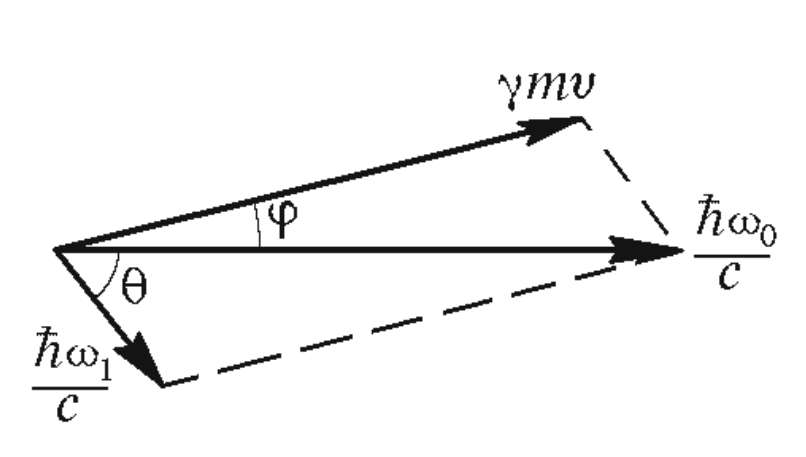
\includegraphics[width=1.0\linewidth]{Screenshot_1}
		\caption{Векторная диаграмма рассеяния \gmm-кванта на электроне}
		\label{fig:screenshot1}
	\end{wrapfigure}

	Эффект Комптона -- увеличение длины волны рассеянного излучения по сравнению с падающим -- интерпретируется как результат упругого соударения двух частиц: \gmm-кванта	(фотона) и свободного электрона. Пусть электрон до соударения покоился (его энергия равна энергии покоя $ m c^2 $), а \gmm-квант имел начальную энергию $ \hbar \omega_0 $ и импульс $ \hbar \omega_0 / c $. После соударения электрон приобретает энергию $ \gamma m c^2 $ и импульс $ \gamma m v $, где $ \gamma = (1- \left(v/c\right)^2)^{-1/2} $, а \gmm-квант рассеивается на некоторый угол $ \theta $ по отношению к первоначальному направлению движения. Энергия и импульс	\gmm-кванта становятся соответственно равными $ \hbar \omega_1 $ и $ \hbar \omega_1 / c $.
	
	Запишем для рассматриваемого процесса ЗСЭ и ЗСИ:
	\begin{gather*}\label{key}
		m c^2 + \hbar \omega_0 = \gamma m c^2 +\hbar \omega_1,\\
		\dfrac{\hbar \omega_0}{c} = \gamma m v \cos \phi + \dfrac{\hbar \omega_1}{c} \cos \theta,\\
		\gamma m v \sin \phi = \dfrac{\hbar \omega_0}{c} \sin \theta.
	\end{gather*}

	Решая совместно эти уравнения и переходя от частот $ \omega_0 $ и $ \omega_1 $ к	длинам волн $ \lambda_0 $ и $ \lambda_1 $, нетрудно получить, что изменение длины волны	рассеянного излучения равно
	\begin{equation}\label{eq:Комптон}
		\lambda_1 - \lambda_0 = \dfrac{h}{m c}\left(1- \cos \theta \right) = \Lambda_к \left(1- \cos \theta \right),
	\end{equation}
	где $$ \Lambda_к = \dfrac{h}{m c} = 2.42\cdot 10^{-10}\; см $$ называется комптоновской длиной волны электрона.
	
	В приведенном выводе электрон в атоме считается свободным. Для	\gmm-квантов с энергией в несколько десятков, а тем более сотен кэВ,	связь электронов в атоме, действительно,	мало существенна, так как энергия их связи в легких атомах не превосходит нескольких кэВ, а для большинства электронов еще меньше.
	
	\subsection{Расчётные формулы}
	
	Основной целью данной работы является проверка соотношения \eqref{eq:Комптон}. Применительно к условиям нашего опыта формулу \eqref{eq:Комптон} следует	преобразовать от длин волн к энергии \gmm-квантов. Как нетрудно показать, соответствующее выражение имеет вид
	\begin{equation}\label{eq:Комптон_нормир}
		\dfrac{1}{\epsilon(\theta)} - \dfrac{1}{\epsilon_0} = 1- \cos(\theta).
	\end{equation}
	Здесь $ \epsilon_0 = E_0/(m c^2) $  -- нормированная энергия \gmm-квантов, падающих на рассеиватель, $ \epsilon(\theta) $ — выраженная в тех же единицах энергия квантов, испытавших комптоновское рассеяние на угол $\theta$, $ m $ -- масса электрона.
	
	\section{Оборудование и инструментальные погрешности}
		
	Схема экспериментальной установки отображена на рис. \ref{fig:screenshot2}.	
	\begin{figure}
		\centering
		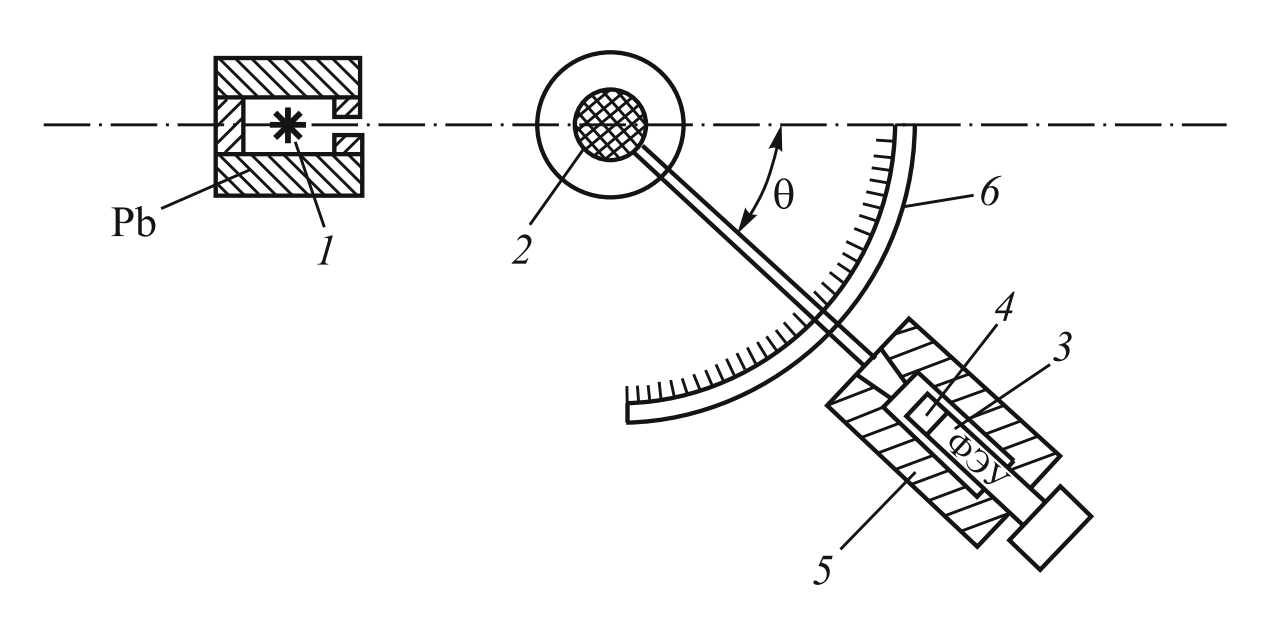
\includegraphics[width=0.7\linewidth]{Screenshot_2}
		\caption{Схема экспериментальной установки}
		\label{fig:screenshot2}
	\end{figure}
	Сформированный коллиматором узкий пучок \gmm-квантов попадает на графитовую мишень. Кванты, испытавшие комптоновское рассеяние в мишени, регистрируются сцинтилляционным счетчиком, состоящим из сцинтиллятора и ФЭУ, работающего от высоковольтного источника напряжения. Сигнал, генерируемый ФЭУ, обрабатывается АЦП компьютера, и соответствующий график выводится на экран.
		
	В работе используются:
	\begin{itemize}
		\equip{Источник \gmm-излучения \isotope{Cs}{137} в свинцовом коллиматоре}
		\Equip{Фотоэлектронный умножитель на градуированном подвижном кронштейне}{1}{^\circ}
		\Equip{Компьютер с 10-разрядным АЦП}{1}{канал}
	\end{itemize}
	
	\section{Результаты измерений и обработка данных}
	
	Запишем формулу \eqref{eq:Комптон_нормир} в удобном виде:
	\begin{equation}\label{eq:Комптон_число}
		\dfrac{1}{N(\theta)} - \dfrac{1}{N(0)} = 1- \cos(\theta).
	\end{equation}
	Здесь $ N(\theta) $ -- номер канала.
	Представим экспериментальные результаты в виде графика на рис. \ref{fig:graph1}, откладывая по оси абсцисс $ 1- \cos(\theta) $, а по оси ординат --- $ {1}/{N(\theta)} $.
	\begin{figure}
		\centering
		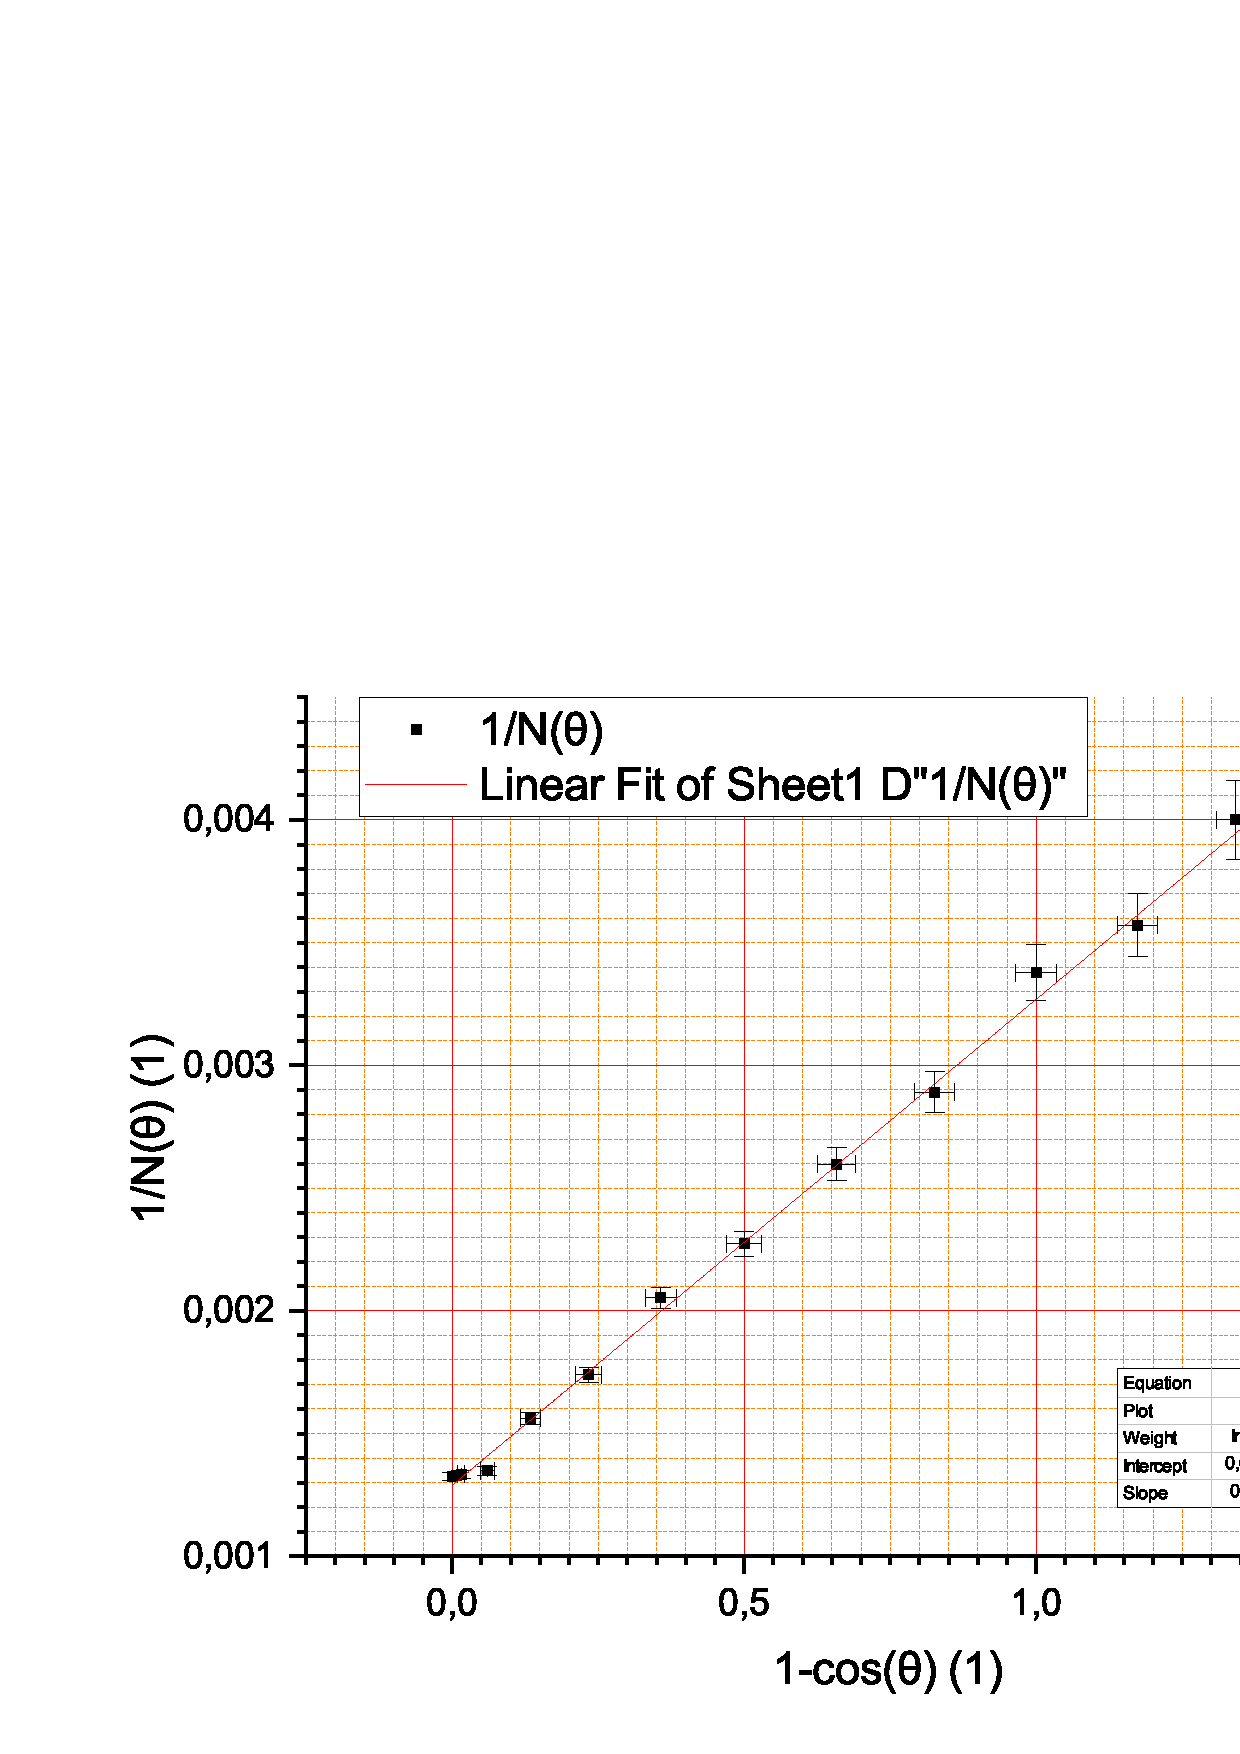
\includegraphics[width=0.8\linewidth]{Graph1}
		\caption{График зависимости $\frac{1}{N} = f(1-\cos \theta)$}
		\label{fig:graph1}
	\end{figure}
	Заметим, что данные плохо ложатся на прямую. Это в первую очередь может быть связано с погрешностью определения пика <<на глаз>>, а также с недостаточной экспозицией при получении спектров. 
	
	По данным графика, уравнение прямой имеет вид\[y = (198\pm 5)\times 10^{-5} x + (129\pm 1)\times 10^{-5}.\]
	Отсюда \[N_{наил}(0) = 775\pm 6\]
	\[\dfrac{1}{N_{наил}(90^\circ)} = (327\pm 5)\times 10^{-5}\]
	\[N_{наил}(90^\circ) = 306\pm 5\]
	
	Исходя из этих данных определим энергию покоя частицы, на которой происходит комптоновское рассеяние (по всем признакам -- электрон):
	\[m c^2 = E_\gamma \dfrac{N(90^\circ)}{N(0)-N(90^\circ)} = 662\times 10^3\times \dfrac{306}{775-306} = 450\pm 20 \; кэВ \]
	Это значение существенно не совпадает с табличным для энергии покоя электрона, что может быть связано как с неточным проведением эксперимента, так и с тем, что электрон  в составе атома не является свободным, поэтому исходная формула \eqref{eq:Комптон} не является достаточно точной в данном случае.	
	
	
	\subsection{Оценка погрешностей}
	Оценка погрешностей проводится при помощи пакета \emph{Wolfram Mathematica} по общей формуле:
	\begin{equation}\label{eq:погрешности}
		\Delta_{u(x, y, z, \ldots)}^2 = f'^2_{x} \Delta_x^2 + f'^2_y \Delta_y^2 + f'^2_z \Delta_z^2 + \ldots,
	\end{equation}
	где $ \Delta_i $ -- случайные или инструментальные погрешности величины $ i $.
	В частности, при расчёте энергии покоя электрона применяется формула
	\begin{equation*}\label{key}
		\Delta_{m c^2} = \sqrt{\frac{E_\gamma^2 \left(N(90)^2 \Delta _{N(0)}^2+N(0)^2 \Delta _{N(90)}^2\right)}{\left(N(0)-N(90)\right){}^4}}
	\end{equation*}
	Для значений $ N(\theta) $ изначальную погрешность в 1 канал пришлось увеличить до 10 каналов, так как определение точки пика затруднительно. Частично можно было исправить ситуацию увеличением времени экспозиции или при помощи компьютерной аппроксимации пиков. Также в этом опыте не была учтена погрешность, вызываемая перепадами напряжения на динодах ФЭУ.
	
	\section{Вывод}
	
	По результатам работы, исследовали эффект Комптона на графитовом образце с помощью сцинтилляционного спектрометра. Выяснили зависимость  энергии рассеянного \gmm-кванта от угла рассеяния, а также определили по порядку величины энергию покоя электрона.
			\newpage
	\appendix
	\section{Необработанные результаты опытов}
	
	<<Сырые>> данные, полученные по результатам опытов, представлены в табл. \ref{tab:raw}.
		
	% Please add the following required packages to your document preamble:
	% \usepackage{multirow}
	\begin{table}[h]
		\centering
		\begin{tabular}{|l|l|l|l|}
			\hline
			Угол $\theta$, $^\circ$ & $\Delta \theta$, $^\circ$ & Канал $N$ & $\Delta N$                \\ \hline
			0                       & \multirow{13}{*}{$\pm 1$} & 755       & \multirow{13}{*}{$\pm 1$} \\ \cline{1-1} \cline{3-3}
			10                      &                           & 750       &                           \\ \cline{1-1} \cline{3-3}
			20                      &                           & 742       &                           \\ \cline{1-1} \cline{3-3}
			30                      &                           & 613       &                           \\ \cline{1-1} \cline{3-3}
			40                      &                           & 594       &                           \\ \cline{1-1} \cline{3-3}
			50                      &                           & 487       &                           \\ \cline{1-1} \cline{3-3}
			60                      &                           & 423       &                           \\ \cline{1-1} \cline{3-3}
			70                      &                           & 385       &                           \\ \cline{1-1} \cline{3-3}
			80                      &                           & 346       &                           \\ \cline{1-1} \cline{3-3}
			90                      &                           & 296       &                           \\ \cline{1-1} \cline{3-3}
			100                     &                           & 280       &                           \\ \cline{1-1} \cline{3-3}
			110                     &                           & 250       &                           \\ \cline{1-1} \cline{3-3}
			120                     &                           & 238       &                           \\ \hline
		\end{tabular}
		\caption{Необработанные данные эксперимента}
		\label{tab:raw}
	\end{table}
		

	\begin{thebibliography}{3}
		\bibitem{Siv} Сивухин Д. В. \emph{Общий курс физики. Том 5}, 1989
		\bibitem{chp} Фаддеев М. А., Чупрунов Е. В. \emph{Лекции по атомной физике}, 2008
		\bibitem{tsip} Ципенюк Ю. М. \emph{Квантовая микро- и макрофизика}, 2006
		\bibitem{max} Игошин Ф. Ф., Самарский Ю. А., Ципенюк Ю. М. \emph{ЛАБОРАТОРНЫЙ ПРАКТИКУМ ПО ОБЩЕЙ ФИЗИКЕ. Квантовая физика: Учеб, пособие для вузов}; Под ред. Ципенюка Ю.М.
	\end{thebibliography}
\end{document}